\chapter{Prototyp}
\label{prototyp}

In diesem Kapitel wird auf zunächst auf die Architektur und die verwendeten Technologien näher eingegangen. Anschliessend wird anhand verschiedener Screenshots die Bedienung der Webanwendung erläutert. Der Name der Webanwendung lautet "`Groupfindr"', das zugehörige Logo ist in Abbildung \ref{logo} dargestellt.


\begin{figure}[h]
\centering

\includegraphics{graphiken/logo.png}%
\caption{Logo der "`Groupfindr"' Anwendung (Quelle: Eigene Darstellung)}%
\label{logo}%
\end{figure}


\section{Architektur und Technologien}
\label{architektur_technologie}

Der groupfindr Prototyp demonstriert die technische Machbarkeit einer skalierbaren real-time Anwendung mit socket.io, exploriert die Darstellungs- und Interaktionsmöglichkeiten der interaktiven Grafikbibliothek EaselJS, und verwendet einen Standardstack an Webtechnologien zur Umsetzung einer responsive Webapplikation.
\newline\newline
Die event-basierte Javascript Bibliothek \textit{\href{http://socket.io/}{socket.io}} ermöglicht die bidirektionale Kommunikation zwischen Client und Server in Echtzeit und bildet die Basis für die groupfindr Funktionalität Bewegungen anderer Benutzer in Echtzeit zu verfolgen. Bewegt ein Benutzer seinen Avatar, wird seine neue Position (\verb|pos|) über einen etablierten Websocket (\verb|socket|) vom Client-Browser an den Server emittiert: \verb|socket.emit('updatepos', pos);|. Der Server reagiert auf den updatepos Event mit dem in Listing 1 gezeigten Callback. Bei der Positionüberprüfung wird festgestellt ob der Benutzer durch die Positionsänderung soeben eine Gruppe verlassen oder betreten hat. Anschliessend wird die neue Position (\verb|newPos|) an alle Benutzer im selben Raum gesendet.

\begin{verbatim}
socket.on('updatepos', function (pos) { 
  // ... 
  // Broadcast new position to all other player in the same room 
  app.io.to(pos.roomname).emit('update', newPos); 
  // ... 
}
\end{verbatim}

Eine Herausforderung mit Echzeitkommunikation dieser Art ist die Sicherstellung einer konsistenten Sicht über alle verbundenen Benutzer. Durch die häufigen parallelen Updates können leicht Logikfehler im Event-Handling entstehen, die beispielsweise dazu führten, dass einzelne Benutzer dupliziert wurden. Des Weiteren hat die Terminologie von Räumen (rooms) für etwas Verwirrung gesorgt, da dieser Begriff sowohl in der technischen (als socket.io Namensraum) als auch in der konzeptionellen (als virtuellen Raum in dem sich Gruppen bilden) Domäne existiert.
\newline\newline
Die in CreateJS enthaltene Javascript Bibliothek EaselJS verwenden wir zur dynamischen Darstellung des Raum Canvas und insbesondere zur Animation des beweglichen Benutzer-Avatars. Dafür bietet EaselJS einen eleganten Weg über sogennante SpriteSheets wie Abbildung X illustriert. Abbildung \ref{create_sprite} zeigt wie diese einzelne Bilder oder eine Abfolge von Bildern für Bewegungen in bestimmte Richtungen mit einer konfigurierbaren Geschwindigkeit (0.4) konfiguriert werden können. Eine nennenswerte Herausforderung war die korrekte relative Berechnung der Positionkoordinaten beim skalieren des Raum Canvas. 

\begin{figure}[h]
\centering
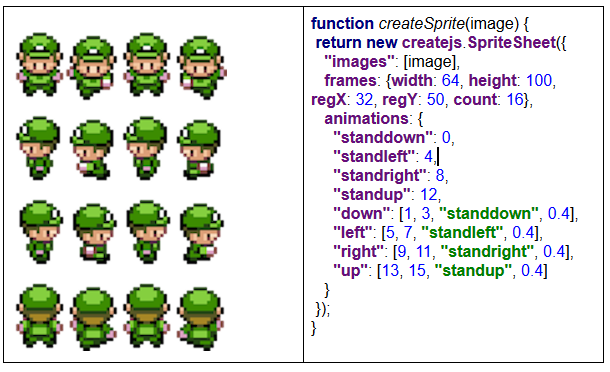
\includegraphics{graphiken/create_sprite.png}%
\caption{Groupfindr - Darstellung des Benutzer Avatars (Quelle: Eigene Darstellung)}%
\label{create_sprite}%
\end{figure}

Groupfindr verwendet einen Standardstack an Webtechnologien zur Umsetzung einer response Webapplikation. Serverseitig kommt Node.js, Express, und die templating Engine Jade zum Einsatz. Die Websocket Verbingungen zwischen Client und Server werden durch socket.io abstrahiert. Clientseitig verwenden wir Bootstrap, CSS, und Javascript mit den Bibliotheken EaselJS, jsPDF, und JQuery.
\newline\newline
Die ausklappbare Chatbox am unteren Bildrand (siehe Abbildung \ref{groupfindr_einfaerbung-chat}) als Einfallstor für Injection Attacken auf alle Benutzer im gleichen Raum dienen. Chatnachrichten erlauben die Verwendung von HTML Tags (z.B. \verb|<b>html</b>|). Während solch harmlose Formatierungen kein Problem darstellen, lässt sich durch die Verwendung eines HTML Skript-Tags beliebiger Code im Browser aller Benutzer ausführen wie das Beispiel in Abbildung \ref{groupfindr_einfaerbung-chat} zeigt. 
\newline
Das Senden der Chatnachricht \verb|<script>window.location = "https://google.com";</script>| leitet alle Benutzer im gleichen Raum unmittelbar auf die Google Website weiter. Sicherheitskritische Attacken dieser Art lassen sich verhindern, indem der Server jede Chatnachricht überprüft und bevor der Weiterleitung an andere Benutzer alle HTML Elemente entsprechend escaped.

\section{How To}
\label{how_to}

Auf der Startseite der Groupfindr Web Applikation (\textit{\href{https://groupfindr.herokuapp.com/}{https://groupfindr.herokuapp.com/}}) kann der Benutzer Benutzername und Raum auswählen (siehe Abbildung \ref{groupfindr_einstieg-gruppenerstellung}). Existierende Räume werden ihm dabei als Dropdown-Auswahl zur Verfügung gestellt. Sobald ein Benutzer einen virtuellen Raum (dargestellt als rechteckige begehbare Fläche) betritt, erhält er einen Avatar zugewiesen (siehe Abbildung \ref{groupfindr_einstieg-gruppenerstellung}). Im virtuellen Raum kann der Benutzer seinen Avatar über Pfeiltasten, per Maus, oder Touch-freundlich per Drag’n’Drop bewegen. Dabei kann jeder Benutzer die Laufwege aller Benutzer im gleichen Raum in Echtzeit mitverfolgen.

\begin{figure}[h]
\centering
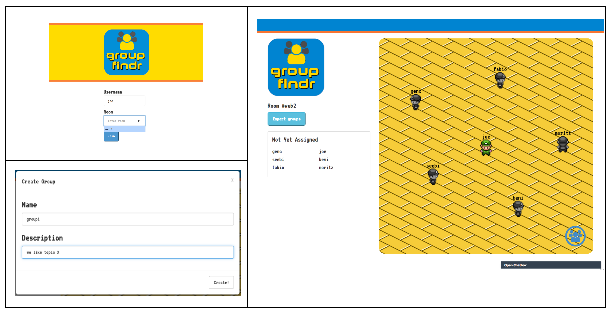
\includegraphics{graphiken/groupfindr_einstieg-gruppenerstellung.png}%
\caption{Groupfindr - Einstieg \& Gruppenerstellung (Quelle: Eigene Darstellung)}%
\label{groupfindr_einstieg-gruppenerstellung}%
\end{figure}


\begin{figure}[h]
\centering
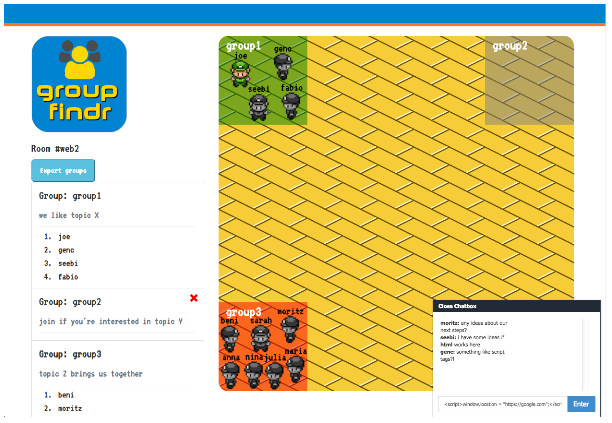
\includegraphics{graphiken/groupfindr_einfaerbung-chat.png}%
\caption{Groupfindr - Einfärbung der Gruppen (Quelle: Eigene Darstellung)}%
\label{groupfindr_einfaerbung-chat}%
\end{figure}

Solange noch freie Plätze auf dem Canvas bestehen (in diesem Prototyp aus Darstellunggründen auf 7 begrenzt), kann jeder Benutzer über den blauen Gruppenbutton im Canvas eine neue Gruppe mit Namen und Beschreibung erstellen. Jeder Benutzer kann einer Gruppe betreten indem er seinen Avatar in das Feld der Gruppe seiner Wahl bewegt (siehe Abbildung \ref{groupfindr_einstieg-gruppenerstellung}). Gruppen mit optimaler Mitgliederanzahl (4-6) werden dabei grün eingefärbt, solche mit zu vielen Mitgliedern sind an der roten Einfärbung schnell zu erkennen, siehe Abbildung \ref{groupfindr_einfaerbung-chat}. Jeder Benutzer kann leere Gruppen wieder löschen um Platz für weitere Gruppen zu schaffen. Die aktuellen Gruppeneinteilungen sind jederzeit in einer textuellen Übersicht, links neben dem Canvas einsehbar. Diese Übersicht lässt sich am Ende des Gruppenfindungsprozesses über die Exportfunktion (Export groups) als PDF herunterladen.